\section{シミュレータを用いた実験}
まずは,新たに作成したネットワークで経路を正しく選択できるかシミュレータを用いた実験により調査する.
次にオフライン学習を追加で行い,効果を検証する.

\subsubsection{実験装置}
シミュレータに Gazebo\cite{gazebo}を使用する.
ロボットには TurtleBot3 Waffle Pi\cite{turtlebot3}に3つのカメラを追加したモデルを用いる.

\subsubsection{実験環境}
実験環境として\figref{fig:haruyama_cit3f}に示す,千葉工業大学2号館3階を模した環境を使用する.
経路の選択を行う場所として\figref{fig:haruyama_cit3f}の A, Bの分岐路を対象に行う.
\figref{fig:select_pattern}に示すように,A,B の各分岐路で経路に侵入するパターンは 3 つ,また脱出するパターンがつ 2 つあることから合計 12 回の経路選択を行うことができる.

\begin{figure}
  \centering
  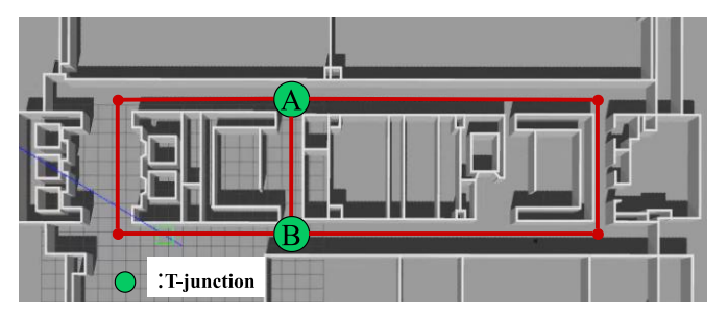
\includegraphics[width=130mm]{images/pdf/haruyama/cit3f.pdf}
  \caption[Experimental environment]{Experimental environment(Quoted from \cite{haruyama2022})}
  \label{fig:haruyama_cit3f}
\end{figure}

\begin{figure}
  \centering
  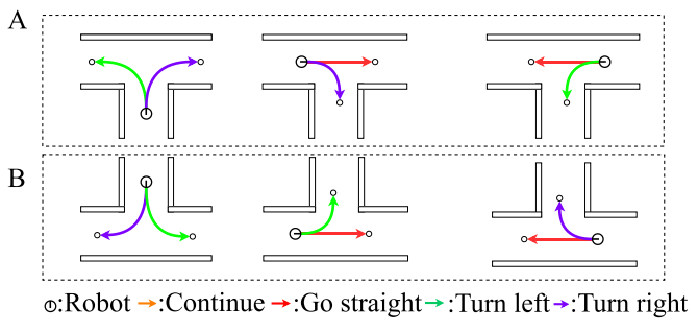
\includegraphics[width=130mm]{images/pdf/haruyama/select_pattern.pdf}
  \caption[Selecting a path the T-junction]{Selecting a path the T-junction(Quoted from \cite{haruyama2022})}
  \label{fig:select_pattern}
\end{figure}
 
\clearpage
\subsubsection{実験方法}
\figref{fig:fujiwara_route}に示す経路を, a から f の順番で走行しながら,模倣学習を行う.
データセットの収集には,藤原ら\cite{fujiwara2023}が提案している,学習データの不均衡を改善する手法,学習時の積極的な蛇行を行う手法を採用する.
テスト時は,学習器の出力で壁に衝突することなく,分岐路の先の経由点に到達することができれば成功とする.
オフライン学習に使用するデータセットは,a から f の順番で走行しながらオンライン学習を行った際に作成されるものを使用する.
オフライン学習のパラメータとして,バッチサイズはオンライン学習と同様の 8 でデータセットからランダムにデータを抽出し,epoch数は 10 とする.
実験では,学習とテストを繰り返し 10 回行う.

\begin{figure}
  \centering
  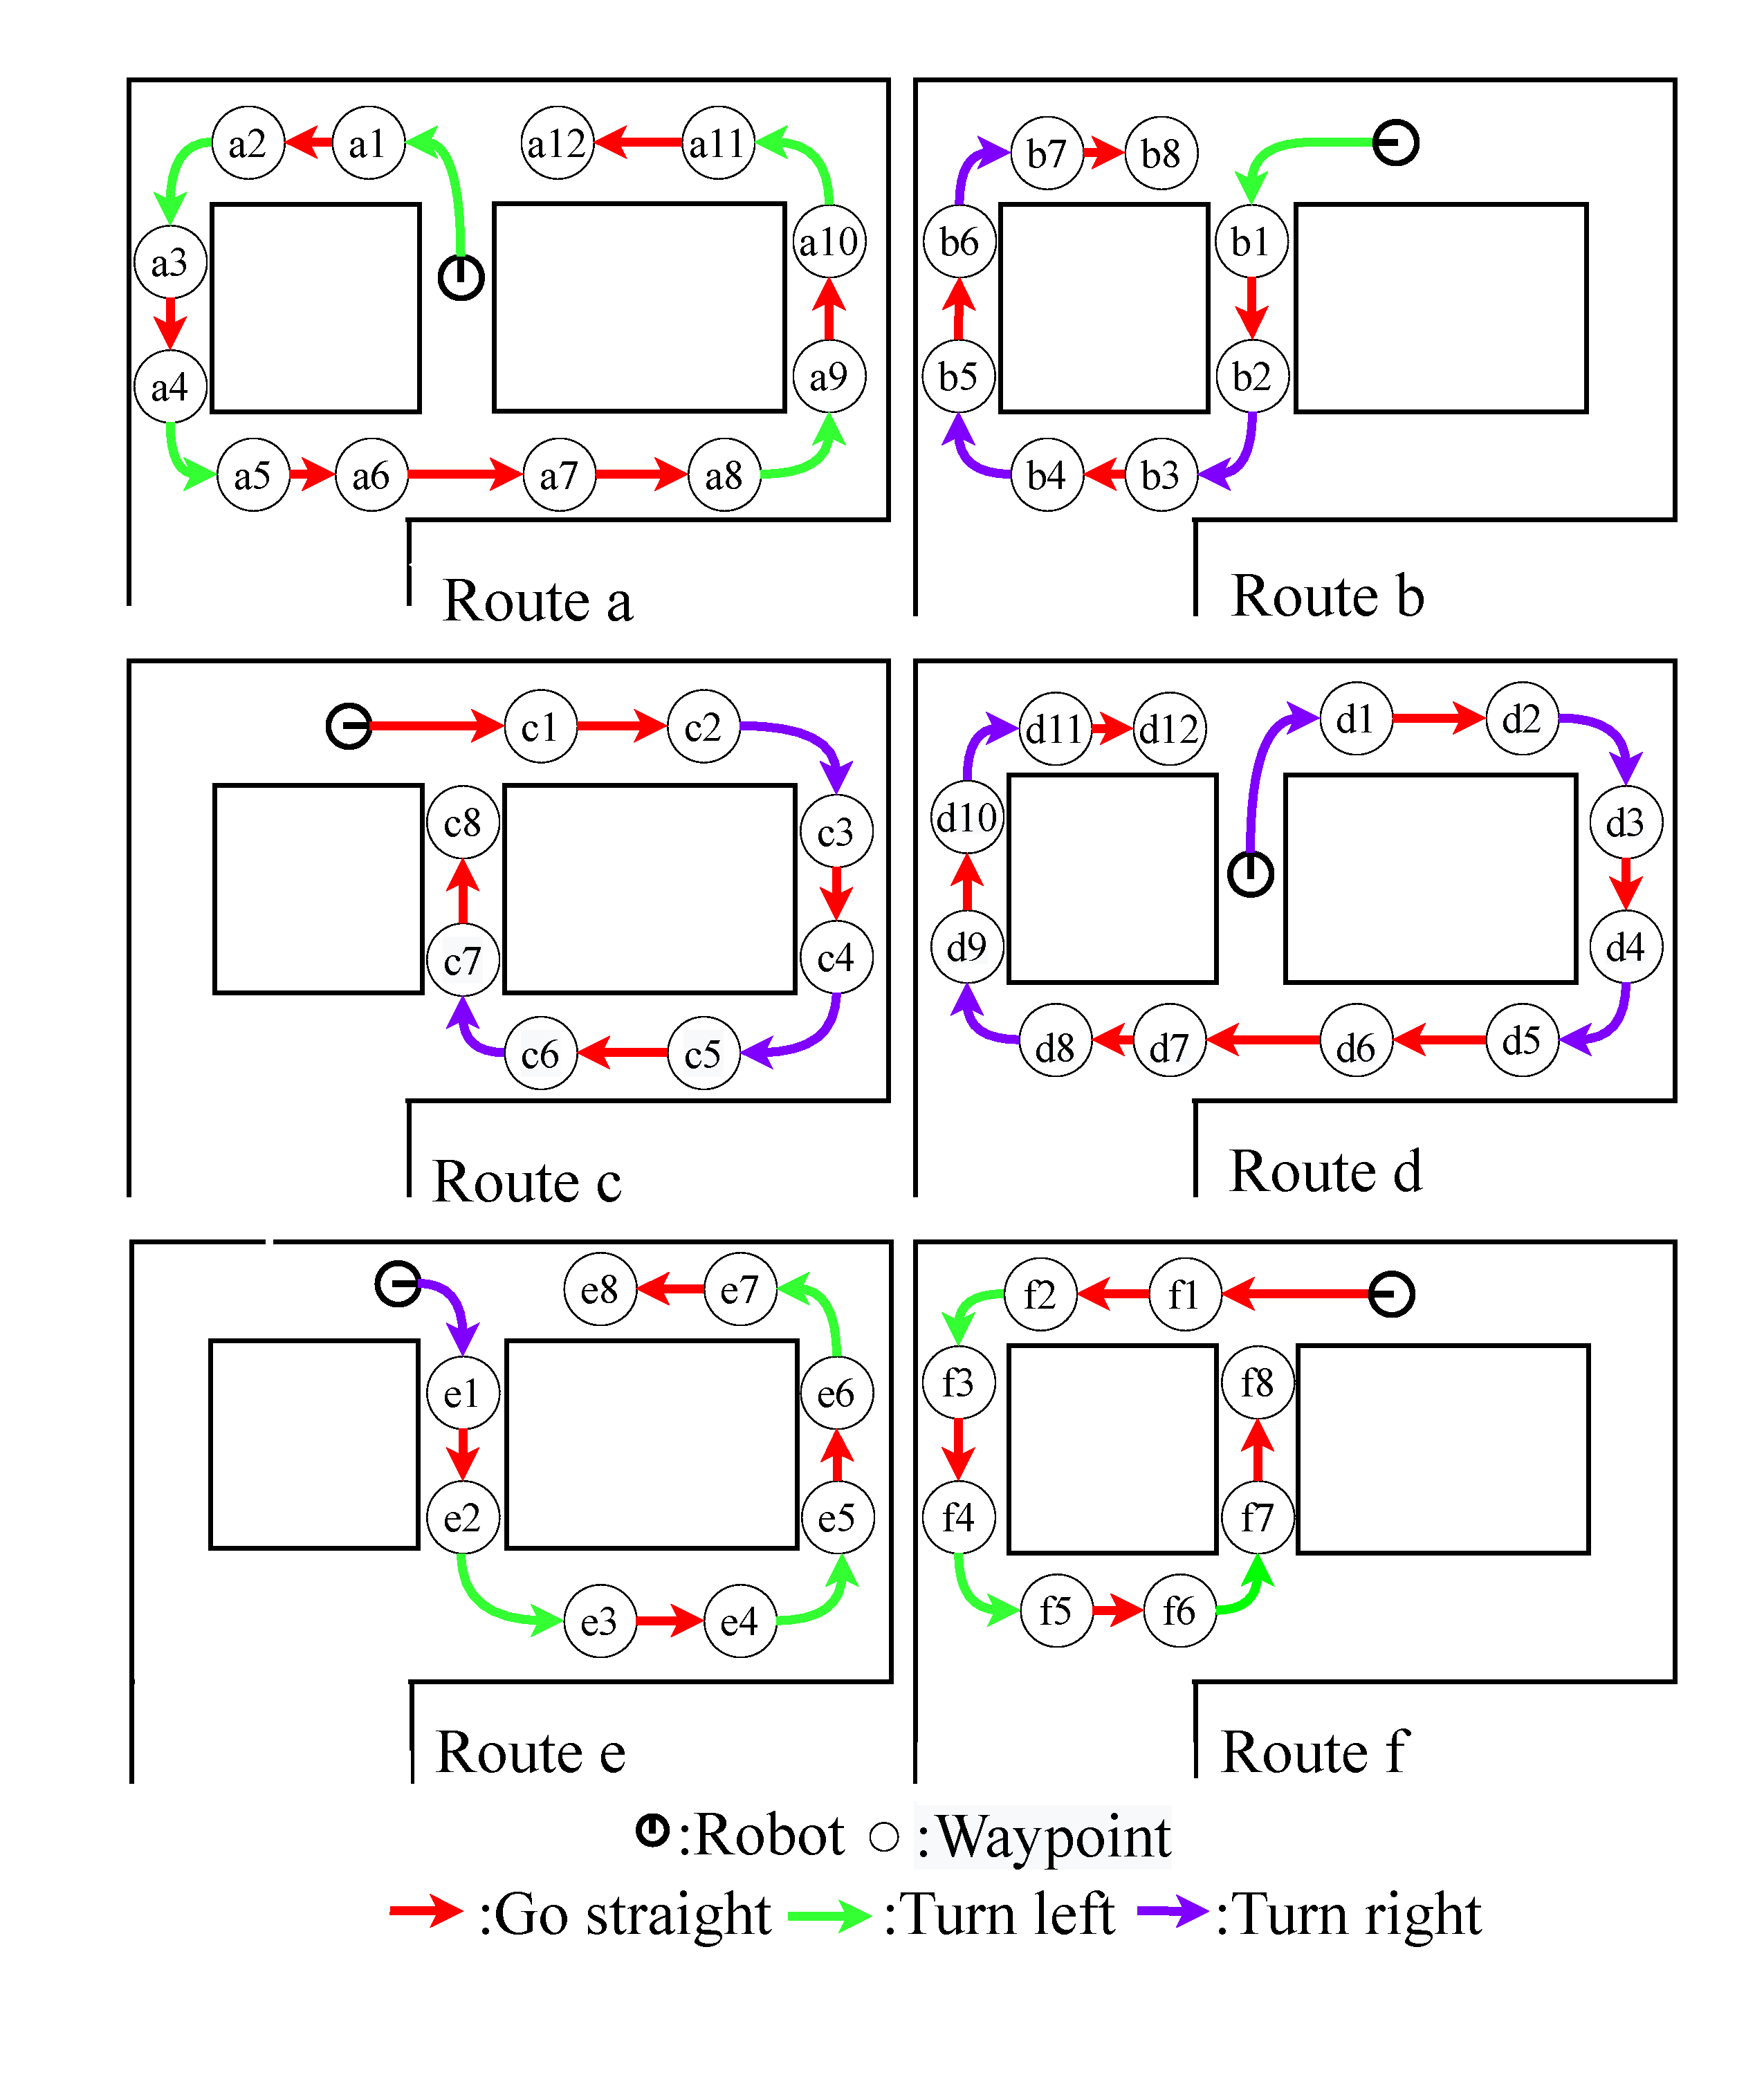
\includegraphics[width=130mm]{images/pdf/fujiwara/route.pdf}
  \caption[Route for experiment]{Route for experiment(Quoted from \cite{fujiwara2023})}
  \label{fig:fujiwara_route}
\end{figure}

\clearpage
\subsubsection{実験結果}
\tabref{tab:result}に結果を示す.
表では,春山らが使用していたネットワークを Previous method としている.
そして新たなネットワークを使用した実験を Branched とした.

新たに作成したネットワークでも,経路を正しく選択することが確認できた.
step数が 10000 の場合は,先行研究の手法と比較すると成功率が上昇した.
しかしstep数が 20000 の場合は先行研究と成功率に大きな差は生じなかった.

オフライン学習を併用した場合では,成功率が 20000 step と同等になった.
一方で,オンライン学習の弱点であったルートの後半部分での失敗を減少させることができた.
具体的には Branched で 10000 step の実験を行った際に一番失敗の多い箇所であった,\figref{fig:fujiwara_route}の Route f の f6 から f7 にかけての経路選択の成功率が向上した.
\tabref{tab:f_result}に,それぞれの実験での f6 から f7 にかけての経路追従の成功率を示す.

これらの結果から,従来の手法では 20000 step 走行しながら学習していたものを, 10000 step まで減らすことができたと言える.
また,ネットワークの変更やオフライン学習は経路選択の可能性を向上させるには有効であると考えられる.

\begin{table}[]
  \centering
  \caption{Success rate}
  \begin{tabular}{lll}
  \hline
  Experiment         & Step + Epoch & Total result     \\ \hline
  Previous method    & 10000        & 109/120 (90.8\%) \\
                     & 20000        & 114/120 (95.0\%) \\ \hline
  Branched           & 10000        & 113/120 (94.2\%) \\ 
                     & 20000        & 115/120 (95.8\%) \\ \hline
  Branched +         & 10000 + 10   & 115/120 (95.8\%) \\ 
  Offline learning   &              &                  \\ \hline
  \end{tabular}
  \label{tab:result}
\end{table}

\begin{table}[]
  \centering
  \caption{Success rate at f6 to f7}
  \begin{tabular}{lll}
  \hline
  Experiment         & Step + Epoch & Total result \\ \hline
  Branched           & 10000        & 5/10         \\ 
                     & 20000        & 7/10         \\ \hline
  Branched +         & 10000 + 10   & 8/10         \\ 
  Offline learning   &              &              \\ \hline
  \end{tabular}
  \label{tab:f_result}
\end{table}